\documentclass[a4paper,10pt,oneside,final,titlepage,onecolumn]{article}

\usepackage{ucs}
\usepackage[portuguese]{babel}
\usepackage[utf8x]{inputenc}
\usepackage[T1]{fontenc}
\usepackage{textcomp}
\usepackage{graphicx}

\usepackage{listings}
\usepackage{color}

\definecolor{dkgreen}{rgb}{0,0.6,0}
\definecolor{gray}{rgb}{0.5,0.5,0.5}
\definecolor{mauve}{rgb}{0.58,0,0.82}

\lstset{frame=tb,
  language=bash,
  aboveskip=3mm,
  belowskip=3mm,
  showstringspaces=false,
  columns=flexible,
  basicstyle={\scriptsize\ttfamily},
  numbers=none,  
  breaklines=true,
  breakatwhitespace=true
  tabsize=3
}



\title{Exercício 3 de MC833 --- Programação em Redes de Computadores}
\author{Raul Rabelo Carvalho, 105607, turma A}



\begin{document}



\maketitle



\section{htons}
\paragraph{}A função \verb|htons| faz parte de um conjunto de funções usadas para converter um inteiro, tanto de 16 bits quanto de 32 bits, entre a \emph{byte order} de rede (\emph{big endian}) e a \emph{byte order} do \emph{host} local, que pode ser \emph{big endian} ou \emph{little endian} a depender da arquitetura. É óbvio que caso a arquitetura do \emph{host} seja \emph{big endian}, nada é feito.
\paragraph{}Especificamente, a função \verb|htons| converte inteiros de 16 bits da \emph{byte order} do \emph{host} para da rede.



\section{Execução com código-fonte não-modificado}
\paragraph{}Não é possível executar o servidor sem alterações no \emph{host} do laboratório do IC (\verb|guns.ic.unicamp.br|), pois a função \verb|bind| não tem permissão para utilizar a porta 10. Esta porta é uma das \emph{well-known ports} e estão bloqueadas para usuários sem privilégios nas máquinas do IC.



\section{Resolvendo o problema do bind}
\paragraph{}Alterando-se a porta empregada para 1234, tanto em \verb|client.c| quanto em \verb|server.c|, resolve-se o problema do servidor não conseguir reservar para si uma das \emph{well-known ports}. No entanto, o cliente não consegue se conectar a esta porta, provavelmente devido àlguma política de bloqueio de portas no roteador dos laboratórios.
\paragraph{}Fazendo uma segunda alteração para a porta 10000, o servidor consegue reservar a porta e executar normalmente, e o cliente consegue conectar-se a esta porta e comunicar-se com o servidor, como na figura \ref{exec-local}.
\begin{figure}[!ht]
  \caption{Execução local.}
  \centering
  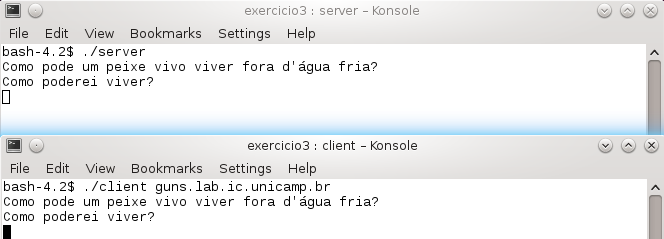
\includegraphics[width=117mm]{exec-local.png}
  \label{exec-local}
\end{figure}
\paragraph{}Também foi possível executar o servidor no \emph{host} local e o cliente na máquina \verb|xaveco| via \verb|ssh|, executado com o comando \verb|./client guns.lab.ic.unicamp.br|.
\begin{figure}[!ht]
  \caption{Execução remota.}
  \centering
  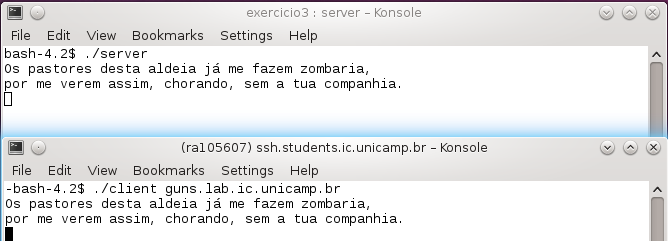
\includegraphics[width=117mm]{exec-remota.png}
  \label{exec-remota}
\end{figure}



\section{Múltiplos clientes}



\section{Verificando o uso da rede}
\paragraph{}Pode-se configurar a porta usada no servidor para uma porta disponível no \emph{host} em que ele vá ser executado. Com conhecimento desta porta, se estabelece a conexão entre cliente e servidor normalmente. Em um terceiro \verb|terminal|, executa-se o comando \verb|netstat -tu| e, se a comunicaçao entre cliente e servidor se faz por rede, uma conexão estabelecida com endereço IP do \emph{host} do servidor e a porta TCP empregada estará listada na saída desta ferramenta.
\paragraph{}Como mostrado na figura \ref{netstat}, existe uma conexão estabelecida entre o servidor em \verb|xaveco.lab.ic.unicamp.br|, usando a porta 10101. Foi usado o comando \verb|netstat -tun|, pois a porta 10101, apesar de estar acima de 1024, tem uma aplicação conhecida associada a ela. A conexão em questão está listada na terceira linha da saída do comando \verb|netstat| e um \emph{reverse} \verb|nslookup| foi feito para se confirmar que o endereço IP \verb|143.106.16.163| corresponde ao nome \verb|xaveco.lab.ic.unicamp.br|.
\begin{figure}[!ht]
  \caption{Netstat -tun.}
  \centering
  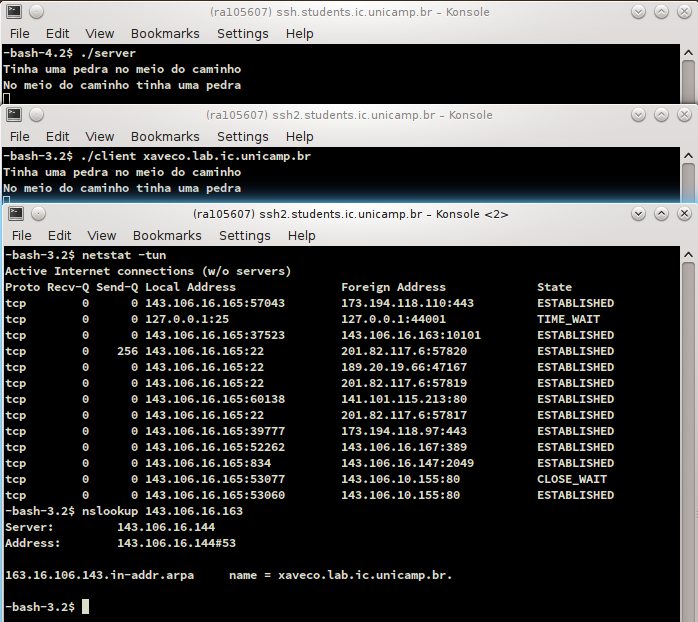
\includegraphics[width=117mm]{netstat.png}
  \label{netstat}
\end{figure}



\section{telnet}

\begin{figure}[!ht]
  \caption{Usando telnet como cliente.}
  \centering
  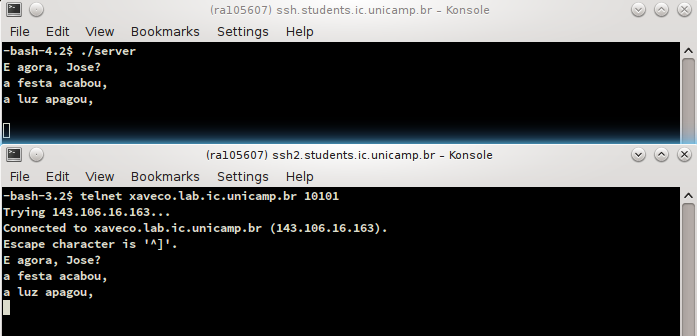
\includegraphics[width=117mm]{telnet.png}
  \label{telnet}
\end{figure}



\end{document}
